\documentclass[paper=letter,fontsize=11pt]{scrartcl} % KOMA-article class
							
\usepackage[english]{babel}
\usepackage[utf8x]{inputenc}
\usepackage{comment} %Para que va a ser ? para comentar
\usepackage[protrusion=true,expansion=true]{microtype}
\usepackage{amsmath,amsfonts,amsthm}     % Math packages
\usepackage{graphicx}                    % Enable pdflatex
\usepackage[svgnames]{xcolor}            % Colors by their 'svgnames'
\usepackage{geometry}
	%\textheight=700px                    % Saving trees ;-)
%\usepackage{url}
\usepackage[colorlinks=true,
linkcolor=blue,
urlcolor=blue]{hyperref}
\usepackage{float}
\usepackage{etaremune}
\usepackage{wrapfig}

\usepackage{attachfile}

\frenchspacing              % Better looking spacings after periods
\pagestyle{empty}           % No pagenumbers/headers/footers

%\addtolength{\voffset}{-40pt}
%\addtolength{\textheight}{20pt}

\setlength\topmargin{0pt}
\addtolength\topmargin{-\headheight}
\addtolength\topmargin{-\headsep}
\setlength\oddsidemargin{0pt}
\setlength\textwidth{\paperwidth}
\addtolength\textwidth{-2in}
\setlength\textheight{\paperheight}
%\addtolength\textheight{-3in}
\addtolength\textheight{-2in}
\usepackage{layout}

%%% Custom sectioning}{sectsty package)
%%% ------------------------------------------------------------
\usepackage{sectsty}

\sectionfont{%			            % Change font of \section command
	\usefont{OT1}{phv}{b}{n}%		% bch-b-n: CharterBT-Bold font
	\sectionrule{0pt}{0pt}{-5pt}{1pt}}

%%% Macros
%%% ------------------------------------------------------------
\newlength{\spacebox}
\settowidth{\spacebox}{8888888888}			% Box to align text
\newcommand{\sepspace}{\vspace*{1em}}		% Vertical space macro

\newcommand{\MyName}[1]{ % Name
		\Huge \usefont{OT1}{phv}{b}{n} \hfill #1
		\par \normalsize \normalfont}
		
\newcommand{\MySlogan}[1]{ % Slogan}{optional)
		\large \usefont{OT1}{phv}{m}{n}\hfill \textit{#1}
		\par \normalsize \normalfont}

\newcommand{\NewPart}[2]{\section*{\uppercase{#1} \small \normalfont #2}}

\newcommand{\NewParttwo}[1]{
		\noindent \huge \textbf{#1}
        \normalsize \par}



\newcommand{\PersonalEntry}[2]{\small
		\noindent\hangindent=2em\hangafter=0 % Indentation
		\parbox{\spacebox}{        % Box to align text
		\textit{#1}}		       % Entry name}{birth, address, etc.)
		\small\hspace{1.5em} #2 \par}    % Entry value

\newcommand{\SkillsEntry}[2]{      % Same as \PersonalEntry
		\noindent\hangindent=2em\hangafter=0 % Indentation
		\parbox{\spacebox}{        % Box to align text
		\textit{#1}}			   % Entry name}{birth, address, etc.)
		\hspace{1.5em} #2 \par}    % Entry value	
		
\newcommand{\EducationEntry}[4]{
		\noindent \textbf{#1} \hfill      % Study
		\colorbox{White}{%
			\parbox{6em}{%
			\hfill\color{Black}#2}} \par  % Duration
		\noindent \textit{#3} \par        % School
		\noindent\hangindent=2em\hangafter=0 \small #4 % Description
		\normalsize \par}

\newcommand{\WorkEntry}[5]{
		\noindent \textbf{#1}
        \noindent \small \textit{#2}
        \hfill      % Study
        \colorbox{White}{%
			\parbox{6em}{%
			\hfill\color{Black}#3}} \par  % Duration
		\noindent \textit{#4} \par        % School
		\noindent\hangindent=2em\hangafter=0 \small #5 % Description
		\normalsize \par}

\newcommand{\Language}[2]{
		\noindent \textbf{#1}
        \noindent \small \textit{#2}}
        
\newcommand{\Text}[1]{\par       
		\noindent \small #1 
		\normalsize \par}
        
\newcommand{\Textlong}[4]{
		\noindent \textbf{#1} \par
        \sepspace
        \noindent \small #2
        \par\sepspace      
		\noindent \small #3
        \par\sepspace      
		\noindent \small #4
        \normalsize \par}
	    
              

\newcommand{\PaperEntry}[7]{
		\noindent #1, ``\href{#7}{#2}", \textit{#3} \textbf{#4}, #5 (#6).}


\newcommand{\ArxivEntry}[3]{
		\noindent #1, ``\href{http://arxiv.org/abs/#3}{#2}", \textit{{cond-mat/}#3}.}
        
\newcommand{\BookEntry}[4]{
		\noindent #1, ``\href{#3}{#4}", \textit{#3}.}
        
\newcommand{\FundingEntry}[5]{
        \noindent #1, ``#2", \$#3 (#4, #5).}

\newcommand{\TalkEntry}[4]{
		\noindent #1, #2, #3 #4}

\newcommand{\ThesisEntry}[5]{
		\noindent #1 -- #2 #3 ``#4" \textit{#5}}

\newcommand{\CourseEntry}[3]{
		\noindent \item{#1: \textbf{#2} \\ #3}}

%%% Begin Document
%%% ------------------------------------------------------------
\begin{document}



%%% you can upload a photo and include it here...
%%\begin{wrapfigure}{l}{0.1\textwidth}
%%	\vspace*{-2em}
%%		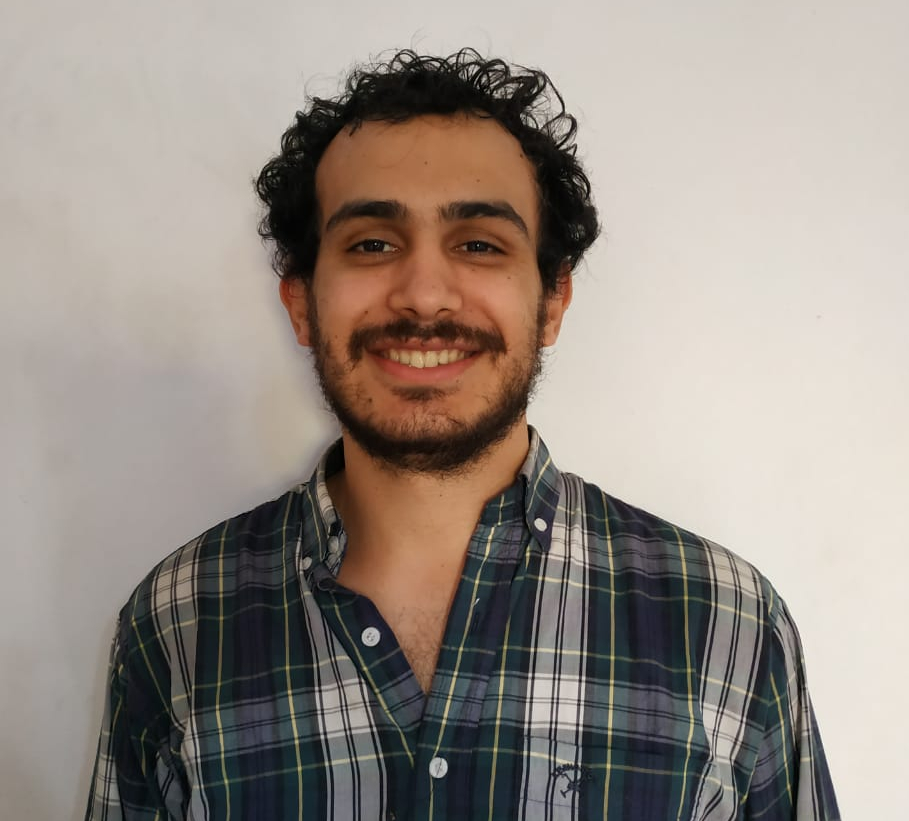
\includegraphics[width=0.25\textwidth]{pic4.jpeg}
%%\end{wrapfigure}

\MyName{Amadio, Camilo Leonel}
\MySlogan{Curriculum Vit\ae\ (\today)}

\sepspace
\sepspace
\sepspace
%%% Personal details
%%% ------------------------------------------------------------
\NewPart{}{}

\PersonalEntry{Phone:}{+ 54 221 155945496}
\PersonalEntry{Mail:}{\href{mailto:camiloamadio57@gmail.com}{camiloamadio57@gmail.com}}
\PersonalEntry{Nationality:}{Argentinian.}
\PersonalEntry{Born:}{27/04/1995}


\NewPart{About me}{}

\sepspace

I'm a physicist that love system modelling and the creation of end to end products, from deploy the databases/servers/pipelines to serving and monitoring of the models. 
\\


I think that building a ml based product is necessarily more than just a model, one of my favourites quotes is:

`` Moreover, 72\% of a cohort of organizations that began AI pilots before 2019 have not
been able to deploy even a single application in production.
 Algorithmia’s survey of the state of enterprise machine
learning found that 55\% of companies surveyed have not deployed an ML model."

- \href{https://cloud.google.com/resources/mlops-whitepaper?hl=es}{Practitioners Guide to MLOps: A framework for continuous delivery and automation of machine learning}


%%% Work experience
%%% ------------------------------------------------------------
\NewPart{Current work}{}

\sepspace




\WorkEntry{Teacher ``Machine Learning II" :}
{}{\hbox{Feb. 2022 - Present}}
{UBA, Buenos Aires, Argentina.}
{
\begin{itemize}
	\item \href{https://docs.google.com/document/d/1OxThFRjgF_6rssui72ZJRAYMpe7QeRiKPYT9XMUfbI8/edit?usp=sharing}{Link} to the official documentation  written by me (in spanish).
	\item Master in artificial intelligence at largest university in Argentina.
	\item We teach how to have a successful ML product.
\end{itemize}
}

\sepspace


\NewPart{Work Experience}{}

\sepspace

\WorkEntry{Data Scientist at Wildlife Studios:}
{}{\hbox{Oct. 2021 - Oct. 2022}}
{Buenos Aires, Argentina.}
{
\begin{itemize}
	\item I've worked at Ads Monetization Department.
	\item Specialized in selling ads through waterfalls.
	\item Specialized in campaings to reduce ANRs through blocking ads.
\end{itemize}
}



\WorkEntry{Data Scientist at Accenture:}
{}{\hbox{Aug. 2019 - Oct. 2021}}
{Buenos Aires, Argentina.}
{
\begin{itemize}
	\item Build, train and deploy machine learning models.
	\item Data mining, simulations and profiling in Python.
\end{itemize}
}

\sepspace

\WorkEntry{Paid Student Teaching Assistant:}
{}{\hbox{Feb. 2018 - Feb. 2020}}
{Facultad de Ingeniería (FI), Universidad Nacional de La Plata (UNLP), La Plata, Argentina.}
{
Teaching assistant in ”Linear Algebra” and ”Electromagnetism”, second year engineering subjects.
}

\sepspace

\NewPart{PROGRAMMING LANGUAGES AND TOOLS}{}

\begin{itemize}
\item Python
\item SQL
\item Power BI
\item Machine Learning Modelling: Classification, Forecasting, Churn prediction, Clustering, Segmentation.
\item Machine Learning Deployment: VMs, DB, Lambda functions, Buckets
\item A/B testing
\item Statistics
\end{itemize}



%%% Work experience
%%% ------------------------------------------------------------
\NewPart{Education}{}

\EducationEntry{Master in Physics: } {2013-2021}{Facultad de Ciencias Exactas (FCE), \\ Universidad Nacional de La Plata (UNLP), La Plata, Argentina.}{

{\href{http://www.exactas.unlp.edu.ar/licenciatura_en_fisica}{Link}} to the webpage of the degree (in spanish).
\begin{itemize}
\item{Grade Point Average: 9.21 \\ {\href{https://drive.google.com/drive/folders/1je8C0gsbGixCF5rJo3fzQaqo1cs2mjX7?usp=sharing}{Link}} to the official Academic Transcript (in spanish).}
\item{Master Thesis: Singularities in quantum field theory.}
\end{itemize}

}

\sepspace




%%% LANGUAGES
%%% ------------------------------------------------------------
\NewPart{LANGUAGES}{}

\begin{itemize}
\item \textbf{Spanish:} Mother Tongue.
\item \textbf{English:} Fluent.
\end{itemize}




\begin{comment}


%%% LANGUAGES
%%% ------------------------------------------------------------
\NewPart{Interests and personality}{}

\Text{Sports and outdoor activities, mainly freeride skiing. The last couple of years I have been competing in freeride skiing and been partially living in the Swiss Alps. Through my skiing I have also developed my ski production. My friends and family form my other big interest. I see myself as a happy, outgoing and reliable person. I am a problem solver and no challenge is too big. The result of my work is often better than expected.}




\NewPart{Expected Salary:}{}

\WorkEntry{}{}{}{}{
\begin{itemize}
\item{My expected salary is in the 700 to 800 USD range.}
\end{itemize}
}

\end{comment}


\end{document}
